% 1977 年青海卷第二题：圆 O、直径 AB（水平）、切线 AC（A 处竖直）、弦 CB 交圆于 D，
% 辅助线 AD 为虚线，∠ABC=45° 标在 B 处（按源卷第 1 页布局）
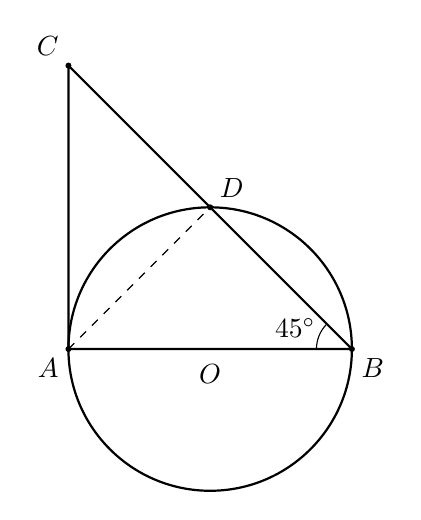
\begin{tikzpicture}[scale=0.9]
  \draw[thick] (0,0) circle (2);
  \coordinate (A) at (-2,0);
  \coordinate (B) at (2,0);
  \coordinate (C) at (-2,4);
  \coordinate (D) at (0,2);
  \draw[thick] (A)--(C)--(B)--cycle;
  \draw[dashed] (A)--(D);
  \fill (A) circle (1.2pt) node[below left] {$A$};
  \fill (B) circle (1.2pt) node[below right] {$B$};
  \fill (C) circle (1.2pt) node[above left] {$C$};
  \fill (D) circle (1.2pt) node[above right] {$D$};
  \node at (0,-0.35) {$O$};
  \draw ([shift={(180:0.5)}]B) arc[start angle=180, end angle=135, radius=0.5];
  \node at (1.2,0.3) {$45^\circ$};
\end{tikzpicture}
